\documentclass[11pt]{article}
\usepackage[margin=1in]{geometry}
\usepackage[T1]{fontenc}
\usepackage{lmodern}
\usepackage{microtype}
\usepackage{amsmath,amssymb}
\usepackage{booktabs}
\usepackage{array}
\usepackage{tabularx}
\usepackage[section]{placeins}
\usepackage[dvipsnames]{xcolor}
\usepackage{graphicx}
\usepackage{hyperref}
\usepackage{xurl}
\usepackage{tikz}
\usetikzlibrary{arrows.meta,positioning,calc,fit}
\usepackage{pgfplots}
\pgfplotsset{compat=1.18}
\usepackage{enumitem}
\usepackage{fancyhdr}
\usepackage{listings}
\usepackage[font=small,labelfont=bf,skip=6pt,singlelinecheck=false]{caption}
\captionsetup[table]{position=above,skip=6pt}
\captionsetup[figure]{position=below,skip=8pt}

\definecolor{fishgreen}{HTML}{0B5D46}
\definecolor{fishlight}{HTML}{EAF4EF}
\definecolor{fishgray}{HTML}{4B5954}
\hypersetup{colorlinks=true, linkcolor=fishgreen, citecolor=fishgreen, urlcolor=fishgreen,
            pdftitle={Bridge, Not Edge: An Independent Re-measurement of KRAKEN v1.1 against SESTINA v1.0},
            pdfauthor={Dylan Nguyen}}
\setlist{topsep=.4\baselineskip,partopsep=0pt,itemsep=2pt,parsep=0pt,leftmargin=*}
\setlist[description]{style=unboxed,leftmargin=0pt,labelsep=0.5em,topsep=\medskipamount,itemsep=\medskipamount,parsep=0pt}
\setlength{\parindent}{1.2em}
\setlength{\parskip}{0pt plus 1pt}
\setlength{\emergencystretch}{3em}
\widowpenalty=10000 \clubpenalty=10000 \displaywidowpenalty=10000 \brokenpenalty=10000
\setlength{\tabcolsep}{4pt}
\renewcommand{\arraystretch}{1.15}
\setlength{\heavyrulewidth}{0.08em}
\setlength{\lightrulewidth}{0.05em}
\newcolumntype{L}{>{\raggedright\arraybackslash}X}
\newcolumntype{R}{>{\raggedleft\arraybackslash}X}
\newcolumntype{Q}[1]{>{\hsize=#1\hsize\raggedright\arraybackslash}X}
\newcolumntype{N}[1]{>{\hsize=#1\hsize\raggedleft\arraybackslash}X}
\newcommand{\ci}[2]{#1\newline{\scriptsize $[#2]$}}
\setcounter{topnumber}{3} \setcounter{totalnumber}{4}
\renewcommand{\topfraction}{0.92} \renewcommand{\textfraction}{0.08} \renewcommand{\floatpagefraction}{0.72}
\pagestyle{fancy} \fancyhf{} \lhead{\small KRAKEN v1.1 against SESTINA v1.0} \cfoot{\thepage}
\renewcommand{\headrulewidth}{0.2pt}
\lstset{basicstyle=\ttfamily\small, breaklines=true, columns=fullflexible, keepspaces=true,
        frame=none, xleftmargin=1.2em, aboveskip=0.6\baselineskip, belowskip=0.6\baselineskip, showstringspaces=false}
\newcommand{\code}[1]{\texttt{#1}}
\newcommand{\flag}[1]{\texttt{-{}-#1}}
\newcommand{\sestina}{\mbox{SESTINA v1.0}}
\newcommand{\kraken}{\mbox{KRAKEN}}
\newcommand{\pct}{\%}

% Generated by research/kraken-check/make_numbers.py -- do not edit.  One macro per number;
% the comment on each line names the artifact it was read from.
\newcommand{\kcMegaMargin}{+2.3466}  % upstream/results/mega_match.json
\newcommand{\kcMegaLo}{+2.2928}  % mega_match.json
\newcommand{\kcMegaHi}{+2.4004}  % mega_match.json
\newcommand{\kcMegaSD}{2.75}  % mega_match.json
\newcommand{\kcMegaSetShare}{63.0}  % mega_match.json
\newcommand{\kcMegaWin}{80.4}  % mega_match.json
\newcommand{\kcMegaWins}{8,041}  % mega_match.json
\newcommand{\kcMegaLosses}{1,959}  % mega_match.json
\newcommand{\kcMegaN}{10,000}  % mega_match.json
\newcommand{\kcMegaDeclKV}{96.5}  % mega_match.json
\newcommand{\kcMegaDeclS}{78.9}  % mega_match.json
\newcommand{\kcMegaAskKV}{51.7}  % mega_match.json
\newcommand{\kcMegaAskS}{48.1}  % mega_match.json
\newcommand{\kcMegaWrongS}{8,442}  % mega_match.json
\newcommand{\kcMegaWrongKV}{1,759}  % mega_match.json
\newcommand{\kcMegaAllocS}{2,775}  % mega_match.json
\newcommand{\kcMegaBridgeRev}{2}  % mega_match.json
\newcommand{\kcUjGames}{10,000}  % upstream/results/mega_match_journal.jsonl
\newcommand{\kcUjDeclPerGameKV}{5.00}  % mega_match_journal.jsonl
\newcommand{\kcUjDeclPerGameS}{4.00}  % mega_match_journal.jsonl
\newcommand{\kcUjWrongPerGameS}{0.844}  % mega_match_journal.jsonl
\newcommand{\kcUjWrongPerGameKV}{0.176}  % mega_match_journal.jsonl
\newcommand{\kcUjUnfinished}{0}  % mega_match_journal.jsonl
\newcommand{\kcUjFallbacks}{0}  % mega_match_journal.jsonl
\newcommand{\kcUpstreamHead}{5da2040}  % upstream/UPSTREAM.txt
\newcommand{\kcPaperNeverMoved}{398}  % kraken.pdf s11.9 (transcribed)
\newcommand{\kcPaperRateRatio}{67}  % kraken.pdf s11.9 (transcribed)
\newcommand{\kcPaperFollowedBoth}{1,927}  % kraken.pdf s11.9 (transcribed)
\newcommand{\kcPaperFollowedBothPct}{19.25}  % kraken.pdf s11.9 (transcribed)
\newcommand{\kcPaperFollowedTakingPct}{3.16}  % kraken.pdf s11.9 (transcribed)
\newcommand{\kcPaperDeclShare}{57}  % kraken.pdf s11.9 (transcribed)
\newcommand{\kcPaperTheirWrongPerGame}{0.844}  % kraken.pdf s11.9 (transcribed)
\newcommand{\kcPaperOurWrongPerGame}{0.176}  % kraken.pdf s11.9 (transcribed)
\newcommand{\kcPaperBridgeBugPrice}{-0.0784}  % kraken.pdf s11.9 (transcribed)
\newcommand{\kcPaperVthreeMargin}{+2.412}  % kraken.pdf abstract (transcribed)
\newcommand{\kcPaperShimDecisions}{329}  % kraken.pdf appendix C (transcribed)
\newcommand{\kcBeliefCertLines}{189--201}  % engine/src/belief.hpp
\newcommand{\kcBeliefPinLine}{200}  % engine/src/belief.hpp
\newcommand{\kcReadmeOffturnGap}{-0.300}  % derived from the README table: both-may minus nobody
\newcommand{\kcEOffturnGap}{+0.111}  % derived: default minus on-turn-only
\newcommand{\kcReadmeNobody}{+2.675}  % engine/external/kraken/kraken/README.md (transcribed)
\newcommand{\kcReadmeBoth}{+2.375}  % kraken/README.md (transcribed)
\newcommand{\kcReadmeOnlyYou}{+1.575}  % kraken/README.md (transcribed)
\newcommand{\kcEDefaultGames}{5,400}  % e1_results.jsonl
\newcommand{\kcEDefaultBlocks}{9}  % e1_results.jsonl
\newcommand{\kcEDefaultWin}{40.3}  % e1_results.jsonl
\newcommand{\kcEDefaultWinLo}{38.3}  % e1_results.jsonl
\newcommand{\kcEDefaultWinHi}{42.3}  % e1_results.jsonl
\newcommand{\kcEDefaultMargin}{-0.648}  % e1_results.jsonl
\newcommand{\kcEDefaultMarginLo}{-0.740}  % e1_results.jsonl
\newcommand{\kcEDefaultMarginHi}{-0.556}  % e1_results.jsonl
\newcommand{\kcEDefaultDeclA}{98.6}  % e1_results.jsonl
\newcommand{\kcEDefaultDeclB}{98.0}  % e1_results.jsonl
\newcommand{\kcEDefaultAskA}{53.8}  % e1_results.jsonl
\newcommand{\kcEDefaultAskB}{56.0}  % e1_results.jsonl
\newcommand{\kcENoootGames}{6,000}  % e1_results.jsonl
\newcommand{\kcENoootBlocks}{10}  % e1_results.jsonl
\newcommand{\kcENoootWin}{38.7}  % e1_results.jsonl
\newcommand{\kcENoootWinLo}{37.3}  % e1_results.jsonl
\newcommand{\kcENoootWinHi}{40.2}  % e1_results.jsonl
\newcommand{\kcENoootMargin}{-0.759}  % e1_results.jsonl
\newcommand{\kcENoootMarginLo}{-0.842}  % e1_results.jsonl
\newcommand{\kcENoootMarginHi}{-0.676}  % e1_results.jsonl
\newcommand{\kcENoootDeclA}{98.1}  % e1_results.jsonl
\newcommand{\kcENoootDeclB}{98.8}  % e1_results.jsonl
\newcommand{\kcENoootAskA}{51.7}  % e1_results.jsonl
\newcommand{\kcENoootAskB}{53.9}  % e1_results.jsonl
\newcommand{\kcEMirrorGames}{1,200}  % e1_results.jsonl
\newcommand{\kcEMirrorBlocks}{2}  % e1_results.jsonl
\newcommand{\kcEMirrorWin}{50.0}  % e1_results.jsonl
\newcommand{\kcEMirrorWinLo}{50.0}  % e1_results.jsonl
\newcommand{\kcEMirrorWinHi}{50.0}  % e1_results.jsonl
\newcommand{\kcEMirrorMargin}{+0.000}  % e1_results.jsonl
\newcommand{\kcEMirrorMarginLo}{+0.000}  % e1_results.jsonl
\newcommand{\kcEMirrorMarginHi}{+0.000}  % e1_results.jsonl
\newcommand{\kcEMirrorDeclA}{98.7}  % e1_results.jsonl
\newcommand{\kcEMirrorDeclB}{98.7}  % e1_results.jsonl
\newcommand{\kcEMirrorAskA}{60.0}  % e1_results.jsonl
\newcommand{\kcEMirrorAskB}{60.0}  % e1_results.jsonl
\newcommand{\kcEKvSixGames}{3,000}  % e1_results.jsonl
\newcommand{\kcEKvSixBlocks}{5}  % e1_results.jsonl
\newcommand{\kcEKvSixWin}{42.3}  % e1_results.jsonl
\newcommand{\kcEKvSixWinLo}{40.3}  % e1_results.jsonl
\newcommand{\kcEKvSixWinHi}{44.4}  % e1_results.jsonl
\newcommand{\kcEKvSixMargin}{-0.495}  % e1_results.jsonl
\newcommand{\kcEKvSixMarginLo}{-0.608}  % e1_results.jsonl
\newcommand{\kcEKvSixMarginHi}{-0.382}  % e1_results.jsonl
\newcommand{\kcEKvSixDeclA}{98.5}  % e1_results.jsonl
\newcommand{\kcEKvSixDeclB}{97.9}  % e1_results.jsonl
\newcommand{\kcEKvSixAskA}{53.9}  % e1_results.jsonl
\newcommand{\kcEKvSixAskB}{55.7}  % e1_results.jsonl
\newcommand{\kcEVsVsixGames}{3,000}  % e1_results.jsonl
\newcommand{\kcEVsVsixBlocks}{5}  % e1_results.jsonl
\newcommand{\kcEVsVsixWin}{44.1}  % e1_results.jsonl
\newcommand{\kcEVsVsixWinLo}{41.3}  % e1_results.jsonl
\newcommand{\kcEVsVsixWinHi}{46.8}  % e1_results.jsonl
\newcommand{\kcEVsVsixMargin}{-0.440}  % e1_results.jsonl
\newcommand{\kcEVsVsixMarginLo}{-0.650}  % e1_results.jsonl
\newcommand{\kcEVsVsixMarginHi}{-0.230}  % e1_results.jsonl
\newcommand{\kcEVsVsixDeclA}{98.4}  % e1_results.jsonl
\newcommand{\kcEVsVsixDeclB}{98.5}  % e1_results.jsonl
\newcommand{\kcEVsVsixAskA}{55.6}  % e1_results.jsonl
\newcommand{\kcEVsVsixAskB}{56.9}  % e1_results.jsonl
\newcommand{\kcENoootNcGames}{3,000}  % e1_results.jsonl
\newcommand{\kcENoootNcBlocks}{5}  % e1_results.jsonl
\newcommand{\kcENoootNcWin}{41.2}  % e1_results.jsonl
\newcommand{\kcENoootNcWinLo}{39.8}  % e1_results.jsonl
\newcommand{\kcENoootNcWinHi}{42.6}  % e1_results.jsonl
\newcommand{\kcENoootNcMargin}{-0.632}  % e1_results.jsonl
\newcommand{\kcENoootNcMarginLo}{-0.700}  % e1_results.jsonl
\newcommand{\kcENoootNcMarginHi}{-0.564}  % e1_results.jsonl
\newcommand{\kcENoootNcDeclA}{98.0}  % e1_results.jsonl
\newcommand{\kcENoootNcDeclB}{98.8}  % e1_results.jsonl
\newcommand{\kcENoootNcAskA}{52.2}  % e1_results.jsonl
\newcommand{\kcENoootNcAskB}{53.9}  % e1_results.jsonl
\newcommand{\kcELegacyGames}{3,000}  % e1_results.jsonl
\newcommand{\kcELegacyBlocks}{5}  % e1_results.jsonl
\newcommand{\kcELegacyWin}{38.9}  % e1_results.jsonl
\newcommand{\kcELegacyWinLo}{37.4}  % e1_results.jsonl
\newcommand{\kcELegacyWinHi}{40.3}  % e1_results.jsonl
\newcommand{\kcELegacyMargin}{-0.739}  % e1_results.jsonl
\newcommand{\kcELegacyMarginLo}{-0.889}  % e1_results.jsonl
\newcommand{\kcELegacyMarginHi}{-0.590}  % e1_results.jsonl
\newcommand{\kcELegacyDeclA}{97.9}  % e1_results.jsonl
\newcommand{\kcELegacyDeclB}{98.8}  % e1_results.jsonl
\newcommand{\kcELegacyAskA}{51.4}  % e1_results.jsonl
\newcommand{\kcELegacyAskB}{53.6}  % e1_results.jsonl
\newcommand{\kcEVsFcheapGames}{1,800}  % e1_results.jsonl
\newcommand{\kcEVsFcheapBlocks}{3}  % e1_results.jsonl
\newcommand{\kcEVsFcheapWin}{44.1}  % e1_results.jsonl
\newcommand{\kcEVsFcheapWinLo}{38.2}  % e1_results.jsonl
\newcommand{\kcEVsFcheapWinHi}{50.1}  % e1_results.jsonl
\newcommand{\kcEVsFcheapMargin}{-0.506}  % e1_results.jsonl
\newcommand{\kcEVsFcheapMarginLo}{-0.795}  % e1_results.jsonl
\newcommand{\kcEVsFcheapMarginHi}{-0.216}  % e1_results.jsonl
\newcommand{\kcEVsFcheapDeclA}{98.0}  % e1_results.jsonl
\newcommand{\kcEVsFcheapDeclB}{98.4}  % e1_results.jsonl
\newcommand{\kcEVsFcheapAskA}{55.6}  % e1_results.jsonl
\newcommand{\kcEVsFcheapAskB}{57.0}  % e1_results.jsonl
\newcommand{\kcEVsVfiveGames}{1,800}  % e1_results.jsonl
\newcommand{\kcEVsVfiveBlocks}{3}  % e1_results.jsonl
\newcommand{\kcEVsVfiveWin}{43.4}  % e1_results.jsonl
\newcommand{\kcEVsVfiveWinLo}{40.3}  % e1_results.jsonl
\newcommand{\kcEVsVfiveWinHi}{46.5}  % e1_results.jsonl
\newcommand{\kcEVsVfiveMargin}{-0.416}  % e1_results.jsonl
\newcommand{\kcEVsVfiveMarginLo}{-0.675}  % e1_results.jsonl
\newcommand{\kcEVsVfiveMarginHi}{-0.156}  % e1_results.jsonl
\newcommand{\kcEVsVfiveDeclA}{98.6}  % e1_results.jsonl
\newcommand{\kcEVsVfiveDeclB}{98.2}  % e1_results.jsonl
\newcommand{\kcEVsVfiveAskA}{56.9}  % e1_results.jsonl
\newcommand{\kcEVsVfiveAskB}{58.2}  % e1_results.jsonl
\newcommand{\kcEVsVfourGames}{1,800}  % e1_results.jsonl
\newcommand{\kcEVsVfourBlocks}{3}  % e1_results.jsonl
\newcommand{\kcEVsVfourWin}{43.9}  % e1_results.jsonl
\newcommand{\kcEVsVfourWinLo}{39.1}  % e1_results.jsonl
\newcommand{\kcEVsVfourWinHi}{48.7}  % e1_results.jsonl
\newcommand{\kcEVsVfourMargin}{-0.407}  % e1_results.jsonl
\newcommand{\kcEVsVfourMarginLo}{-0.613}  % e1_results.jsonl
\newcommand{\kcEVsVfourMarginHi}{-0.201}  % e1_results.jsonl
\newcommand{\kcEVsVfourDeclA}{98.0}  % e1_results.jsonl
\newcommand{\kcEVsVfourDeclB}{98.4}  % e1_results.jsonl
\newcommand{\kcEVsVfourAskA}{53.1}  % e1_results.jsonl
\newcommand{\kcEVsVfourAskB}{54.5}  % e1_results.jsonl
\newcommand{\kcEKvSixPairedGames}{3,000}  % e1_results.jsonl
\newcommand{\kcEKvSixPairedBlocks}{5}  % e1_results.jsonl
\newcommand{\kcEKvSixPairedWin}{39.6}  % e1_results.jsonl
\newcommand{\kcEKvSixPairedWinLo}{37.0}  % e1_results.jsonl
\newcommand{\kcEKvSixPairedWinHi}{42.1}  % e1_results.jsonl
\newcommand{\kcEKvSixPairedMargin}{-0.649}  % e1_results.jsonl
\newcommand{\kcEKvSixPairedMarginLo}{-0.784}  % e1_results.jsonl
\newcommand{\kcEKvSixPairedMarginHi}{-0.514}  % e1_results.jsonl
\newcommand{\kcEKvSixPairedDeclA}{98.4}  % e1_results.jsonl
\newcommand{\kcEKvSixPairedDeclB}{98.0}  % e1_results.jsonl
\newcommand{\kcEKvSixPairedAskA}{53.6}  % e1_results.jsonl
\newcommand{\kcEKvSixPairedAskB}{55.8}  % e1_results.jsonl
\newcommand{\kcESestinaGames}{17,400}  % e1_results.jsonl
\newcommand{\kcESestinaBlocks}{29}  % e1_results.jsonl
\newcommand{\kcESestinaWinMin}{38.7}  % e1_results.jsonl
\newcommand{\kcESestinaWinMax}{41.2}  % e1_results.jsonl
\newcommand{\kcESestinaMarginMin}{-0.759}  % e1_results.jsonl
\newcommand{\kcESestinaMarginMax}{-0.632}  % e1_results.jsonl
\newcommand{\kcETotalGames}{33,000}  % e1_results.jsonl
\newcommand{\kcETotalBlocks}{55}  % e1_results.jsonl
\newcommand{\kcEDefaultSEsFromClaim}{75}  % derived: (claim - cell) / block SE
\newcommand{\kcENoootSEsFromClaim}{84}  % derived: (claim - cell) / block SE
\newcommand{\kcECardlessShift}{+0.127}  % derived: nooot_nocardless - nooot
\newcommand{\kcEKvSixDiffBlocks}{5}  % e1_results.jsonl
\newcommand{\kcEKvSixDiff}{-0.015}  % derived: kv6 - kraken on identical blocks
\newcommand{\kcEKvSixDiffLo}{-0.026}  % derived
\newcommand{\kcEKvSixDiffHi}{-0.005}  % derived
\newcommand{\kcEDefaultForcedPerGame}{0.029}  % e1_results.jsonl
\newcommand{\kcEDefaultForcedAcc}{71.8}  % e1_results.jsonl
\newcommand{\kcEDefaultFallbackBound}{0.016}  % derived: 2 x forced/game x (1 - forced accuracy)
\newcommand{\kcENoootForcedPerGame}{0.406}  % e1_results.jsonl
\newcommand{\kcENoootForcedAcc}{91.8}  % e1_results.jsonl
\newcommand{\kcENoootFallbackBound}{0.067}  % derived: 2 x forced/game x (1 - forced accuracy)
\newcommand{\kcVMaxAbsRho}{0.044}  % derived: parity correlation within a deal, worst over variants
\newcommand{\kcVMaxClusterDiff}{0.003}  % derived: |clustered - unclustered half-width|, worst over variants
\newcommand{\kcEThroughput}{9}  % e1_results.jsonl (median block, 9 threads shared with other runs)
\newcommand{\kcEThreads}{9}  % e1_results.jsonl
\newcommand{\kcVRevTwoGames}{2,000}  % e2_rev2.jsonl
\newcommand{\kcVRevTwoMargin}{+2.446}  % e2_rev2.jsonl
\newcommand{\kcVRevTwoLo}{+2.327}  % e2_rev2.jsonl
\newcommand{\kcVRevTwoHi}{+2.565}  % e2_rev2.jsonl
\newcommand{\kcVRevTwoSetShare}{63.6}  % e2_rev2.jsonl
\newcommand{\kcVRevTwoWin}{81.7}  % e2_rev2.jsonl
\newcommand{\kcVRevTwoDeclS}{78.0}  % e2_rev2.jsonl
\newcommand{\kcVRevTwoVolS}{77.8}  % e2_rev2.jsonl
\newcommand{\kcVRevTwoForcedS}{79.4}  % e2_rev2.jsonl
\newcommand{\kcVRevTwoForcedPerGame}{0.52}  % e2_rev2.jsonl
\newcommand{\kcVRevTwoDeclKV}{96.7}  % e2_rev2.jsonl
\newcommand{\kcVRevTwoAskS}{48.0}  % e2_rev2.jsonl
\newcommand{\kcVRevTwoAskKV}{51.6}  % e2_rev2.jsonl
\newcommand{\kcVRevTwoOwnErr}{0.592}  % e2_rev2.jsonl
\newcommand{\kcVRevTwoAllocErr}{0.285}  % e2_rev2.jsonl
\newcommand{\kcVRevTwoFallbacks}{0}  % e2_rev2.jsonl
\newcommand{\kcVRevTwoUnfinished}{0}  % e2_rev2.jsonl
\newcommand{\kcVDealtGames}{2,000}  % e2_dealthand.jsonl
\newcommand{\kcVDealtMargin}{-0.703}  % e2_dealthand.jsonl
\newcommand{\kcVDealtLo}{-0.828}  % e2_dealthand.jsonl
\newcommand{\kcVDealtHi}{-0.578}  % e2_dealthand.jsonl
\newcommand{\kcVDealtSetShare}{46.1}  % e2_dealthand.jsonl
\newcommand{\kcVDealtWin}{39.5}  % e2_dealthand.jsonl
\newcommand{\kcVDealtDeclS}{96.9}  % e2_dealthand.jsonl
\newcommand{\kcVDealtVolS}{97.5}  % e2_dealthand.jsonl
\newcommand{\kcVDealtForcedS}{93.9}  % e2_dealthand.jsonl
\newcommand{\kcVDealtForcedPerGame}{0.73}  % e2_dealthand.jsonl
\newcommand{\kcVDealtDeclKV}{97.3}  % e2_dealthand.jsonl
\newcommand{\kcVDealtAskS}{54.9}  % e2_dealthand.jsonl
\newcommand{\kcVDealtAskKV}{52.6}  % e2_dealthand.jsonl
\newcommand{\kcVDealtOwnErr}{0.042}  % e2_dealthand.jsonl
\newcommand{\kcVDealtAllocErr}{0.107}  % e2_dealthand.jsonl
\newcommand{\kcVDealtFallbacks}{0}  % e2_dealthand.jsonl
\newcommand{\kcVDealtUnfinished}{0}  % e2_dealthand.jsonl
\newcommand{\kcVDealtPaired}{-3.149}  % e2_dealthand.jsonl vs e2_rev2.jsonl
\newcommand{\kcVDealtPairedLo}{-3.307}  % paired
\newcommand{\kcVDealtPairedHi}{-2.991}  % paired
\newcommand{\kcVDealtPairedN}{2,000}  % paired
\newcommand{\kcVLadderGames}{2,000}  % e2_ladder.jsonl
\newcommand{\kcVLadderMargin}{+2.443}  % e2_ladder.jsonl
\newcommand{\kcVLadderLo}{+2.324}  % e2_ladder.jsonl
\newcommand{\kcVLadderHi}{+2.562}  % e2_ladder.jsonl
\newcommand{\kcVLadderSetShare}{63.6}  % e2_ladder.jsonl
\newcommand{\kcVLadderWin}{81.5}  % e2_ladder.jsonl
\newcommand{\kcVLadderDeclS}{78.1}  % e2_ladder.jsonl
\newcommand{\kcVLadderVolS}{77.8}  % e2_ladder.jsonl
\newcommand{\kcVLadderForcedS}{79.7}  % e2_ladder.jsonl
\newcommand{\kcVLadderForcedPerGame}{0.52}  % e2_ladder.jsonl
\newcommand{\kcVLadderDeclKV}{96.7}  % e2_ladder.jsonl
\newcommand{\kcVLadderAskS}{48.0}  % e2_ladder.jsonl
\newcommand{\kcVLadderAskKV}{51.6}  % e2_ladder.jsonl
\newcommand{\kcVLadderOwnErr}{0.592}  % e2_ladder.jsonl
\newcommand{\kcVLadderAllocErr}{0.284}  % e2_ladder.jsonl
\newcommand{\kcVLadderFallbacks}{0}  % e2_ladder.jsonl
\newcommand{\kcVLadderUnfinished}{0}  % e2_ladder.jsonl
\newcommand{\kcVLadderPaired}{-0.003}  % e2_ladder.jsonl vs e2_rev2.jsonl
\newcommand{\kcVLadderPairedLo}{-0.008}  % paired
\newcommand{\kcVLadderPairedHi}{+0.002}  % paired
\newcommand{\kcVLadderPairedN}{2,000}  % paired
\newcommand{\kcVSeedGames}{2,000}  % e2_seedvary.jsonl
\newcommand{\kcVSeedMargin}{+2.494}  % e2_seedvary.jsonl
\newcommand{\kcVSeedLo}{+2.374}  % e2_seedvary.jsonl
\newcommand{\kcVSeedHi}{+2.614}  % e2_seedvary.jsonl
\newcommand{\kcVSeedSetShare}{63.9}  % e2_seedvary.jsonl
\newcommand{\kcVSeedWin}{82.1}  % e2_seedvary.jsonl
\newcommand{\kcVSeedDeclS}{78.2}  % e2_seedvary.jsonl
\newcommand{\kcVSeedVolS}{77.7}  % e2_seedvary.jsonl
\newcommand{\kcVSeedForcedS}{81.7}  % e2_seedvary.jsonl
\newcommand{\kcVSeedForcedPerGame}{0.50}  % e2_seedvary.jsonl
\newcommand{\kcVSeedDeclKV}{96.6}  % e2_seedvary.jsonl
\newcommand{\kcVSeedAskS}{47.8}  % e2_seedvary.jsonl
\newcommand{\kcVSeedAskKV}{51.7}  % e2_seedvary.jsonl
\newcommand{\kcVSeedOwnErr}{0.579}  % e2_seedvary.jsonl
\newcommand{\kcVSeedAllocErr}{0.281}  % e2_seedvary.jsonl
\newcommand{\kcVSeedFallbacks}{0}  % e2_seedvary.jsonl
\newcommand{\kcVSeedUnfinished}{0}  % e2_seedvary.jsonl
\newcommand{\kcVSeedPaired}{+0.048}  % e2_seedvary.jsonl vs e2_rev2.jsonl
\newcommand{\kcVSeedPairedLo}{-0.066}  % paired
\newcommand{\kcVSeedPairedHi}{+0.162}  % paired
\newcommand{\kcVSeedPairedN}{2,000}  % paired
\newcommand{\kcVDealtSeedGames}{2,000}  % e2_dealtseed.jsonl
\newcommand{\kcVDealtSeedMargin}{-0.653}  % e2_dealtseed.jsonl
\newcommand{\kcVDealtSeedLo}{-0.779}  % e2_dealtseed.jsonl
\newcommand{\kcVDealtSeedHi}{-0.527}  % e2_dealtseed.jsonl
\newcommand{\kcVDealtSeedSetShare}{46.4}  % e2_dealtseed.jsonl
\newcommand{\kcVDealtSeedWin}{40.1}  % e2_dealtseed.jsonl
\newcommand{\kcVDealtSeedDeclS}{96.6}  % e2_dealtseed.jsonl
\newcommand{\kcVDealtSeedVolS}{97.3}  % e2_dealtseed.jsonl
\newcommand{\kcVDealtSeedForcedS}{92.9}  % e2_dealtseed.jsonl
\newcommand{\kcVDealtSeedForcedPerGame}{0.72}  % e2_dealtseed.jsonl
\newcommand{\kcVDealtSeedDeclKV}{97.5}  % e2_dealtseed.jsonl
\newcommand{\kcVDealtSeedAskS}{55.0}  % e2_dealtseed.jsonl
\newcommand{\kcVDealtSeedAskKV}{52.7}  % e2_dealtseed.jsonl
\newcommand{\kcVDealtSeedOwnErr}{0.044}  % e2_dealtseed.jsonl
\newcommand{\kcVDealtSeedAllocErr}{0.121}  % e2_dealtseed.jsonl
\newcommand{\kcVDealtSeedFallbacks}{0}  % e2_dealtseed.jsonl
\newcommand{\kcVDealtSeedUnfinished}{0}  % e2_dealtseed.jsonl
\newcommand{\kcVDealtSeedPaired}{-3.099}  % e2_dealtseed.jsonl vs e2_rev2.jsonl
\newcommand{\kcVDealtSeedPairedLo}{-3.260}  % paired
\newcommand{\kcVDealtSeedPairedHi}{-2.938}  % paired
\newcommand{\kcVDealtSeedPairedN}{2,000}  % paired
\newcommand{\kcVDealtBigGames}{8,000}  % e2_dealthand_big.jsonl
\newcommand{\kcVDealtBigMargin}{-0.570}  % e2_dealthand_big.jsonl
\newcommand{\kcVDealtBigLo}{-0.632}  % e2_dealthand_big.jsonl
\newcommand{\kcVDealtBigHi}{-0.508}  % e2_dealthand_big.jsonl
\newcommand{\kcVDealtBigSetShare}{46.8}  % e2_dealthand_big.jsonl
\newcommand{\kcVDealtBigWin}{41.7}  % e2_dealthand_big.jsonl
\newcommand{\kcVDealtBigDeclS}{96.5}  % e2_dealthand_big.jsonl
\newcommand{\kcVDealtBigVolS}{97.0}  % e2_dealthand_big.jsonl
\newcommand{\kcVDealtBigForcedS}{93.4}  % e2_dealthand_big.jsonl
\newcommand{\kcVDealtBigForcedPerGame}{0.72}  % e2_dealthand_big.jsonl
\newcommand{\kcVDealtBigDeclKV}{97.4}  % e2_dealthand_big.jsonl
\newcommand{\kcVDealtBigAskS}{54.7}  % e2_dealthand_big.jsonl
\newcommand{\kcVDealtBigAskKV}{52.5}  % e2_dealthand_big.jsonl
\newcommand{\kcVDealtBigOwnErr}{0.047}  % e2_dealthand_big.jsonl
\newcommand{\kcVDealtBigAllocErr}{0.123}  % e2_dealthand_big.jsonl
\newcommand{\kcVDealtBigFallbacks}{0}  % e2_dealthand_big.jsonl
\newcommand{\kcVDealtBigUnfinished}{0}  % e2_dealthand_big.jsonl
\newcommand{\kcVDealtHandMismatch}{0}  % e2_dealthand.jsonl
\newcommand{\kcVDealtBigHandMismatch}{0}  % e2_dealthand_big.jsonl
\newcommand{\kcVLadderCalls}{1,040}  % e2_ladder.jsonl
\newcommand{\kcVRevTwoWrongPct}{22.0}  % e2_rev2.jsonl
\newcommand{\kcVRevTwoVolWrongPct}{22.2}  % e2_rev2.jsonl
\newcommand{\kcPrGames}{120}  % e5_probe.json
\newcommand{\kcPrDecisions}{6,403}  % e5_probe.json
\newcommand{\kcPrNativeSets}{599}  % e5_probe.json
\newcommand{\kcPrOppSets}{481}  % e5_probe.json
\newcommand{\kcPrNativeWins}{73}  % e5_probe.json
\newcommand{\kcPrNativeDecl}{580}  % e5_probe.json
\newcommand{\kcPrNativeWrong}{8}  % e5_probe.json
\newcommand{\kcPrNativeWrongPct}{1.4}  % e5_probe.json
\newcommand{\kcPrCurDecl}{793}  % e5_probe.json
\newcommand{\kcPrCurWrong}{176}  % e5_probe.json
\newcommand{\kcPrCurWrongPct}{22.2}  % e5_probe.json
\newcommand{\kcPrCurAgree}{6,127}  % e5_probe.json
\newcommand{\kcPrCurAgreePct}{95.7}  % e5_probe.json
\newcommand{\kcPrCurOnly}{239}  % e5_probe.json
\newcommand{\kcPrCurOnlyWrong}{158}  % e5_probe.json
\newcommand{\kcPrCurOnlyOwn}{134}  % e5_probe.json
\newcommand{\kcPrCurNativeOnly}{26}  % e5_probe.json
\newcommand{\kcPrCurBothDiff}{11}  % e5_probe.json
\newcommand{\kcPrCurAsk}{4,141}  % e5_probe.json
\newcommand{\kcPrCurAskPct}{72.2}  % e5_probe.json
\newcommand{\kcPrDealtDecl}{673}  % e5_probe.json
\newcommand{\kcPrDealtWrong}{38}  % e5_probe.json
\newcommand{\kcPrDealtWrongPct}{5.6}  % e5_probe.json
\newcommand{\kcPrDealtAgree}{6,310}  % e5_probe.json
\newcommand{\kcPrDealtAgreePct}{98.5}  % e5_probe.json
\newcommand{\kcPrDealtOnly}{93}  % e5_probe.json
\newcommand{\kcPrDealtOnlyWrong}{30}  % e5_probe.json
\newcommand{\kcPrDealtOnlyOwn}{22}  % e5_probe.json
\newcommand{\kcPrDealtNativeOnly}{0}  % e5_probe.json
\newcommand{\kcPrDealtBothDiff}{0}  % e5_probe.json
\newcommand{\kcPrDealtAsk}{4,815}  % e5_probe.json
\newcommand{\kcPrDealtAskPct}{84.0}  % e5_probe.json
\newcommand{\kcPrAskCompared}{5,733}  % e5_probe.json
\newcommand{\kcPrFreshFirst}{360}  % e5_probe_fresh.json
\newcommand{\kcPrFreshFirstCur}{360}  % e5_probe_fresh.json
\newcommand{\kcPrFreshFirstDealt}{360}  % e5_probe_fresh.json
\newcommand{\kcPrFreshDealtWrongPct}{5.7}  % e5_probe_fresh.json
\newcommand{\kcPrFreshNativeWrongPct}{1.4}  % e5_probe_fresh.json
\newcommand{\kcPrFreshDealtOnly}{91}  % e5_probe_fresh.json
\newcommand{\kcPrFreshDealtAskPct}{84.0}  % e5_probe_fresh.json
\newcommand{\kcPrFreshDealtNativeOnly}{0}  % e5_probe_fresh.json
\newcommand{\kcPrFreshDealtBothDiff}{0}  % e5_probe_fresh.json
\newcommand{\kcPrFirst}{360}  % e5_probe.json
\newcommand{\kcPrFirstCur}{359}  % e5_probe.json
\newcommand{\kcPrFirstDealt}{359}  % e5_probe.json
\newcommand{\kcPrShimErrors}{0}  % e5_probe.json
\newcommand{\kcIdIdentical}{identical}  % e4_upstream_777001.json vs e1_results.jsonl seed 777001
\newcommand{\kcIdWin}{38.8}  % e1_results.jsonl seed 777001
\newcommand{\kcIdUpWin}{38.8}  % e4_upstream_777001.json
\newcommand{\kcIdSetsA}{4.145}  % e1
\newcommand{\kcIdSetsB}{4.855}  % e1
\newcommand{\kcIdUpSetsA}{4.145}  % e4
\newcommand{\kcIdUpSetsB}{4.855}  % e4
\newcommand{\kcIdAsks}{26,256}  % e1
\newcommand{\kcIdUpAsks}{26,256}  % e4
\newcommand{\kcIdDecl}{2,423}  % e1
\newcommand{\kcIdUpDecl}{2,423}  % e4
\newcommand{\kcBrRequests}{645}  % bridge_kraken_stats.json
\newcommand{\kcBrDecide}{167}  % bridge_kraken_stats.json
\newcommand{\kcBrOffturn}{477}  % bridge_kraken_stats.json
\newcommand{\kcBrErrors}{0}  % bridge_kraken_stats.json
\newcommand{\kcEDefaultSetShare}{46.4}  % e1_results.jsonl


\title{\textbf{Bridge, Not Edge:\\ An Independent Re-measurement of\\ KRAKEN v1.1 against SESTINA v1.0}}
\author{Dylan Nguyen}
\date{2 September 2026}

\begin{document}
\maketitle

\begin{abstract}
\noindent
The KRAKEN v1.1 paper reports that its engine beats \sestina{} by $\kcMegaMargin$ sets per game,
taking \kcMegaSetShare\pct{} of decided sets and \kcMegaWin\pct{} of games over \kcMegaN{} games,
measured in its own arbiter through a process bridge into \sestina{}'s engine. We re-measure the
pairing in both engines. Inside FishLab's arbiter, with KRAKEN hosted exactly as its integration guide
requires, KRAKEN loses under each of the four rule dialects tested: $\kcEDefaultMargin$~$[\kcEDefaultMarginLo, \kcEDefaultMarginHi]$ sets per game under FishLab's rules and
$\kcENoootMargin$ under its own declare-on-turn rule, over \kcESestinaGames{} games. Inside KV's own
arbiter, with their bridge as published, the paper's figure reproduces on fresh deals
($\kcVRevTwoMargin$). The discrepancy is one defect in that bridge: it resets \sestina{} with the hand
it holds \emph{now} where the engine expects the hand it was \emph{dealt}, which corrupts every
legality certificate the belief rebuilds in a half-suit that seat has since gained or lost a card in.
Passing the dealt hand and replaying the identical deals moves the result by $\kcVDealtPaired$~$[\kcVDealtPairedLo, \kcVDealtPairedHi]$ sets per game; KRAKEN then loses in their arbiter too
($\kcVDealtBigMargin$ on \kcVDealtBigGames{} further games), \sestina{}'s declaration accuracy returns
to its native level, and the two arbiters agree under the matched dialect. A decision-level probe shows
the defect on single decisions. The paper's forced-endgame repair and its per-decision seed schedule
are priced and are immaterial. KRAKEN also loses to every earlier release of FishLab's FishBot lineage
from v0.4 upward. Nothing here bears on KRAKEN's internal results; the cross-engine claim, and what the
paper builds on it, does not survive.
\end{abstract}

\section{Introduction}

Two engines for six-player Canadian Fish were written independently in 2026: FishLab, whose
current agent is \sestina{} (developed as FishBot v0.7; \cite{sestina}), and the Python engine of
KV (Kausthubh Veldanda), whose current agent is KRAKEN (v1.0 in code, v1.1 in the paper;
\cite{kraken}; the deployed configuration is the same). In August the two projects
built bridges so that each bot could play inside the other's arbiter, and the KRAKEN paper reports the
result of its exhibition as its cross-engine headline: over \kcMegaN{} games under its rules, KRAKEN
beat \sestina{} by $\kcMegaMargin$ sets per game, won \kcMegaWin\pct{} of games, and declared
half-suits correctly \kcMegaDeclKV\pct{} of the time against \sestina{}'s \kcMegaDeclS\pct{}. The paper
builds a mechanism story on those rows --- \kcPaperDeclShare\pct{} of the margin is attributed to
``knowing when a half-suit is finished'' --- and its package README extends the claim to FishLab's own
dialect, giving \kcReadmeBoth{} sets per game when both sides may declare off-turn.

The size of the claim is what makes it worth checking. \sestina{}'s own evaluation resolves edges of a
few percentage points against its predecessors; an opponent taking four games in five would be a
different order of strength from anything either lineage has produced. The paper is careful about what
the number is: cross-engine strength against one opponent, not a global ranking. But a cross-engine
number is a statement about the bridge as well as the engines, as the paper itself says, and the bridge
is the one component neither project had tested from the other side.

This report does that. It uses four instruments, in the order a sceptic would reach for them:
\begin{enumerate}
\item the same match inside FishLab's arbiter, with KRAKEN played through FishLab's bridge to it
      (Section~\ref{sec:fishlab});
\item a replication inside KV's own arbiter, with their engine, their rules and their bridge, on fresh
      deals (Section~\ref{sec:kv});
\item one-line variants of their bridge, each changing exactly one thing, replayed on identical deals so
      the difference is paired (Section~\ref{sec:variants});
\item a probe that feeds every native \sestina{} decision through KV's own shim and compares the two
      answers decision by decision (Section~\ref{sec:probe}).
\end{enumerate}
Section~\ref{sec:defect} locates the defect in the two code bases and explains why every check the
paper ran passed anyway. Section~\ref{sec:discussion} states what is refuted, what stands, what was
not tested, and what a cross-engine measurement should require of its bridge. Every measurement in this
document is a macro generated from an artifact in \code{research/kraken-check/} by
\code{make\_numbers.py}; the few figures quoted from the KRAKEN paper are transcribed in the same
file under a comment naming their source.

\begin{table}[!ht]
\caption{The claim against the measurements. Left: the paper's headline, from its own results file.
Middle: the same pairing in FishLab's arbiter under FishLab's rules. Right: the same pairing in KV's
arbiter after the one-line repair of Section~\ref{sec:defect}, on fresh deals.}
\label{tab:claims}
\small
\begin{tabularx}{\linewidth}{Q{1.0}Q{1.0}Q{1.0}Q{1.0}}
\toprule
quantity & the paper (KV's arbiter, their bridge) & FishLab's arbiter, FishLab rules & KV's arbiter, bridge repaired \\
\midrule
KRAKEN margin, sets per game & $\kcMegaMargin{}$ $[\kcMegaLo{}, \kcMegaHi{}]$ & $\kcEDefaultMargin{}$ $[\kcEDefaultMarginLo{}, \kcEDefaultMarginHi{}]$ & $\kcVDealtBigMargin{}$ $[\kcVDealtBigLo{}, \kcVDealtBigHi{}]$ \\
KRAKEN share of decided sets & \kcMegaSetShare{}\% & \kcEDefaultSetShare{}\% & \kcVDealtBigSetShare{}\% \\
KRAKEN games won & \kcMegaWin{}\% & \kcEDefaultWin{}\% & \kcVDealtBigWin{}\% \\
SESTINA declaration accuracy & \kcMegaDeclS{}\% & \kcEDefaultDeclB{}\% & \kcVDealtBigDeclS{}\% \\
KRAKEN declaration accuracy & \kcMegaDeclKV{}\% & \kcEDefaultDeclA{}\% & \kcVDealtBigDeclKV{}\% \\
SESTINA ask hit rate & \kcMegaAskS{}\% & \kcEDefaultAskB{}\% & \kcVDealtBigAskS{}\% \\
KRAKEN ask hit rate & \kcMegaAskKV{}\% & \kcEDefaultAskA{}\% & \kcVDealtBigAskKV{}\% \\
games & \kcMegaN{} & \kcEDefaultGames{} & \kcVDealtBigGames{} \\
\bottomrule
\end{tabularx}

\end{table}

\section{The engines, the rules, and the bridges}
\label{sec:setup}

\subsection{Two arbiters, two dialects}

The game, in one paragraph. Fifty-four cards form nine \emph{half-suits} of six; six seats in two
teams of alternating seats are dealt nine cards each. On turn a player \emph{asks} an opponent for a
named card: it is legal only if the asker holds another card of that half-suit and not the card
itself; a hit transfers the card and keeps the turn, a miss passes the turn to the opponent asked. A
team scores a half-suit by \emph{declaring} it: naming which of its own three seats holds each of the
six cards. Every action is public, so the whole hidden state is the deal, and an engine's belief is a
posterior over deals under the constraints the public record implies: a hit pins a card, a miss
excludes a seat, and every ask certifies that the asker held another card of that half-suit at that
moment (a \emph{legality certificate} in what follows). The \emph{arbiter} is the program that runs
the game and scores it; a \emph{bridge} is the code that lets one project's bot play inside the
other's arbiter; a \emph{dialect} is one project's set of choices on the rules the game leaves open.

Both engines implement this game with the no-bluff ask rule and the award rule for misdeclarations: a
declaration that is wrong in any way --- a card with an opponent (an \emph{ownership} error) or all
six within the team but the split misstated (an \emph{allocation} error) --- scores the half-suit for
the other team. (KV's engine scored a right-team, wrong-split declaration as a void until its v0.6; the
paper re-measured everything under the award rule, and every result here uses it.) They differ in four
places that matter to what follows.
\begin{description}
\item[Out-of-turn declaration.] FishLab's default rule lets any seat declare at any moment, and the
      engine polls every seat before every move. KV's baseline lets a seat declare only on its own
      turn (\code{claims\_any\_time = False}). FishLab exposes the latter as \flag{no-out-of-turn}.
\item[Cardless seats.] FishLab lets a cardless seat declare; KV's arbiter makes it pass. FishLab
      exposes the latter as \flag{no-cardless-declare}.
\item[The forced endgame.] When one team is out of cards, FishLab runs a willingness ladder over the
      declaring team: for each half-suit and each seat, at descending confidence thresholds, a seat
      that is willing declares, and only a last resort demands a best guess. Only the willingness bit
      crosses between teammates. In KV's arbiter the mover must claim one half-suit per turn, and the
      bridge chooses which.
\item[What a wrong declaration reveals.] KV's engine reveals the true holders at resolution; FishLab
      reveals nothing.
\end{description}

\subsection{KRAKEN inside FishLab}

FishLab's bridge, \code{engine/src/kv6.hpp}, launches KRAKEN's own package (\code{kraken.decide},
unmodified, under the vendored interpreter) as a line-oriented JSON service, one process per worker
thread. It follows the three requirements KRAKEN's integration guide says a host must get right: every
seat is polled off-turn through KRAKEN's proof-only channel; cards travel as names, with the half-suit
permutation between the two decks derived at start-up from KRAKEN's own \code{\{"op":"cards"\}} table;
and any error reply, illegal move or dead process aborts the run rather than substituting a move. KRAKEN
has no clock, so no timeout is set. Because KRAKEN's belief cannot represent ``resolved, holders
unrevealed'', the engine additionally hands it the true holders after a wrong declaration, out of band
and to no policy of FishLab's --- the one thing FishLab grew for the integration, and a gift to KRAKEN
relative to FishLab's own rule. A full request--reply transcript of one deal is in the artifacts:
\kcBrRequests{} requests (\kcBrDecide{} on-turn decisions, \kcBrOffturn{} off-turn polls),
\kcBrErrors{} error replies. KRAKEN's own consistency checker, which rejects an event stream no deal
could have produced, never fired in any run reported here.

\subsection{SESTINA inside KV's arbiter}
\label{sec:theirbridge}

KV's bridge is \code{fish4/dylan\_v07.py} driving \code{external\_v07/shim\_decide.cpp}, a one-shot
binary compiled from FishLab's headers. It is stateless by construction: for every decision, a fresh
process is started and fed
\begin{lstlisting}
SPEC <the frozen v07 allparams spec>
RULES 9 0 1                 # 9 half-suits, on-turn declaration only, cardless OK
SEAT s
HAND <bitmask>              # the seat's hand NOW (Observation.hand)
SEED <one constant per game>
EV ASK|DECL|PASS ...        # every public event, running counts and score
TURN s
DECIDE TURN                 # or DECIDE FORCED <half-suit> / PASSTO
\end{lstlisting}
and the shim constructs the agent, calls \code{Agent::reset(seat, hand, rules, seed)}, replays the
events through \code{observe()}, and answers one move. \sestina{} is never polled off-turn (their rules
have no such channel); when the mover must declare, the bridge names the first live half-suit the mover holds a card
in and asks for the agent's own proposal on it, falling back to a best guess (this is the paper's
bridge revision~2; revision~1 passed the first
live half-suit outright, and the paper prices the repair at $\kcPaperBridgeBugPrice$ sets per game).
Every proposed move is legality-checked and a failure would be counted; the paper reports zero, and so
does every run here.

\subsection{Versions}

KRAKEN is the package vendored at \code{engine/external/kraken} (v1.0; \code{V06\_DEPLOYED} plus
\code{claim\_forced\_exhaustive=1}). The upstream branch head \code{\kcUpstreamHead} (v1.1) was fetched
and played on the same seed, same rotations and same opponent as the first FishLab block: the results
are \kcIdIdentical{} to the digit (\kcIdUpWin\pct{} against \kcIdWin\pct{} of games,
\kcIdUpSetsA/\kcIdUpSetsB{} against \kcIdSetsA/\kcIdSetsB{} sets, \kcIdUpAsks{} against \kcIdAsks{}
asks, \kcIdUpDecl{} against \kcIdDecl{} declarations). The v1.1 paper says its deployed configuration is
unchanged from v1.0; this confirms it. KV's package was itself called FishBot v0.6 before it became
KRAKEN; the copy vendored at \code{engine/external/kv-fishbot-v06} is an earlier snapshot of that
package whose policy code differs from KRAKEN's in more than the one flag, it is unrelated to FishLab's
own FishBot v0.6, and it is written ``KV FishBot v0.6'' throughout. \sestina{} is the frozen specification in
\code{engine/fishbot\_v07.json}; the \code{allparams} form KV's bridge sends equals their
\code{v07\_spec.txt}. The paper pins FishLab at commit \code{d017fbc}; between that commit and the build
used here the only changes under \code{engine/src/} to any file the policy depends on are two additive
hooks (the true-holder callback above, and factory branches for external bots).

\section{Methods}
\label{sec:methods}

\subsection{The FishLab battery}
\label{sec:m-fishlab}

Each cell is a set of independent blocks of 100 deals played in all six seat rotations (600 games), so
that each policy holds every hand-triple of a deal exactly three times and the deal's luck cancels.
Each block has its own seed and is one invocation of \code{fish match} with \flag{json}; the row it
returns, with its exact \code{argv}, is one line of \code{e1\_results.jsonl}. A cell's estimate is the
mean over its blocks and its interval is a Student~$t$ interval on the block means, which is
deal-clustered by construction. Cells: KRAKEN against \sestina{} under FishLab's default rules, under
\flag{no-out-of-turn} (KRAKEN's dialect), under both that and \flag{no-cardless-declare}, and
under \flag{legacy}; KRAKEN against KRAKEN as a symmetry control; KV FishBot v0.6 against \sestina{}, once on its own seeds and once on the seeds of the default
KRAKEN cell so that the two packages are compared on identical deals; and KRAKEN against FishBot v0.6,
F-cheap (v0.6 with search), v0.5 and v0.4 to place it on this repository's ladder. \kcETotalBlocks{} blocks, \kcETotalGames{} games. Throughput was
about \kcEThroughput{} games per second on \kcEThreads{} threads while the other batteries ran
alongside.

\subsection{Replication in KV's arbiter}
\label{sec:m-kv}

The driver reproduces the design of their \code{scripts4/mega\_match.py} (fetched from upstream and
kept under \code{upstream/scripts4/}): KRAKEN's \code{V06\_DEPLOYED} against three copies of
\code{dylan\_v07}, the award rule, each deal played from both seat parities, their 600-ply cap, one
JSON row per game. It runs their engine and their bridge
unmodified, from the vendored package, with the shim compiled from this repository's headers; only the
seeds are fresh. Each row additionally records, per side, asks and hits, declarations and their
correctness, whether each declaration was forced (the mover had no legal ask), and the class of each
wrong declaration: \emph{ownership} (an opponent held a card of the half-suit) or \emph{allocation}
(the declaring team held all six and named the wrong split). Bridge fallbacks and unfinished games are
counted; both are zero in every row. Intervals in KV's arbiter are normal, $\pm 1.96$ standard errors
on per-game margins; the two parities of a deal are nearly uncorrelated (worst $|\rho| =
\kcVMaxAbsRho$ over the six runs) and deal-clustered half-widths agree with them to within
\kcVMaxClusterDiff{} sets.

\subsection{Bridge variants}
\label{sec:m-variants}

Four variants of their bridge were run on the same deal seeds and agent seeds as the baseline, so
that per-game differences are paired (three change one thing; the fourth combines two repairs), and a
fifth run repeats the repaired bridge on fresh deals. Each subclasses their \code{DylanV07}:
\begin{description}
\item[dealt hand.] \code{HAND} is the hand as dealt, recovered by walking the seat's public transfers
      newest-first from the current hand (a card taken by a successful ask is removed, one lost is
      restored, one retired by a declaration is restored to the seat that held it). Every decision also
      replays the result forward and checks that it reproduces the current hand;
      \kcVDealtHandMismatch{} mismatches occurred in \kcVDealtGames{} games.
\item[ladder.] When the mover must declare, it runs FishLab's forced ladder over every live half-suit
      (voluntary proposal, then willingness at the engine's descending thresholds, then the most
      confident best guess), through a shim extended with one command. \kcVLadderCalls{} forced
      decisions went through it.
\item[seed.] The per-decision agent seed varies with the history length, so the fresh process does not
      restart the same random stream at every decision.
\item[dealt hand and seed.] Both repairs.
\item[dealt hand, fresh deals.] The dealt-hand bridge on \kcVDealtBigGames{} new games, unpaired.
\end{description}

\subsection{The decision probe}
\label{sec:m-probe}

\code{agree\_probe.cpp} wraps native \sestina{} in FishLab's arbiter under KV's rules (declare on
turn only) against KRAKEN. At each of its own on-turn decisions the wrapper also serialises the position
exactly as \code{dylan\_v07.py} does and asks KV's shim binary twice --- once with the current hand,
once with the hand as dealt --- sending the native agent's exact seed (their bridge masks its seed to
63 bits; the probe does not, because the seed is not what is under test). It records whether
the shim declares when the native agent does, whether the declarations match, whether the asks match,
and, using the true hands it has access to as the arbiter, whether each hypothetical declaration
would have been right. The first decision of a game is a special case: the fresh shim process and the
native agent then have identical random state, so if the serialisation is faithful they must answer
identically. The probe was run twice, once with the native agents reused across deals as the
production harness reuses them and once with them rebuilt for every game, because \sestina{}'s own
report documents a rare cross-deal residual in reused agents (its \S12.6).

\section{Results}

\subsection{FishLab's arbiter}
\label{sec:fishlab}

\begin{table}[!ht]
\caption{Every cell of the FishLab battery. Blocks of 100 deals $\times$ 6 rotations; intervals are
Student~$t$ on block means. ``F-cheap'' is FishBot v0.6 with \sestina{}'s search switched on.}
\label{tab:fishlab}
\small
\begin{tabularx}{\linewidth}{Q{0.95}Q{1.0}Q{1.45}N{0.75}N{0.8}N{1.15}N{0.9}}
\toprule
A & B & rules & games & A wins & sets A$-$B per game & decl.\ acc.\ A\,/\,B (\%) \\
\midrule
KRAKEN & SESTINA & FishLab default & \kcEDefaultGames{} & \kcEDefaultWin{}\% & \ci{$\kcEDefaultMargin{}$}{\kcEDefaultMarginLo{},\,\kcEDefaultMarginHi{}} & \kcEDefaultDeclA{}\,/\,\kcEDefaultDeclB{} \\
KRAKEN & SESTINA & declare on turn only & \kcENoootGames{} & \kcENoootWin{}\% & \ci{$\kcENoootMargin{}$}{\kcENoootMarginLo{},\,\kcENoootMarginHi{}} & \kcENoootDeclA{}\,/\,\kcENoootDeclB{} \\
KRAKEN & SESTINA & on turn only, no cardless declaration & \kcENoootNcGames{} & \kcENoootNcWin{}\% & \ci{$\kcENoootNcMargin{}$}{\kcENoootNcMarginLo{},\,\kcENoootNcMarginHi{}} & \kcENoootNcDeclA{}\,/\,\kcENoootNcDeclB{} \\
KRAKEN & SESTINA & legacy dialect & \kcELegacyGames{} & \kcELegacyWin{}\% & \ci{$\kcELegacyMargin{}$}{\kcELegacyMarginLo{},\,\kcELegacyMarginHi{}} & \kcELegacyDeclA{}\,/\,\kcELegacyDeclB{} \\
\midrule
KRAKEN & KRAKEN & FishLab default (control) & \kcEMirrorGames{} & \kcEMirrorWin{}\% & \ci{$\kcEMirrorMargin{}$}{\kcEMirrorMarginLo{},\,\kcEMirrorMarginHi{}} & \kcEMirrorDeclA{}\,/\,\kcEMirrorDeclB{} \\
\midrule
KRAKEN & FishBot v0.6 & FishLab default & \kcEVsVsixGames{} & \kcEVsVsixWin{}\% & \ci{$\kcEVsVsixMargin{}$}{\kcEVsVsixMarginLo{},\,\kcEVsVsixMarginHi{}} & \kcEVsVsixDeclA{}\,/\,\kcEVsVsixDeclB{} \\
KRAKEN & F-cheap & FishLab default & \kcEVsFcheapGames{} & \kcEVsFcheapWin{}\% & \ci{$\kcEVsFcheapMargin{}$}{\kcEVsFcheapMarginLo{},\,\kcEVsFcheapMarginHi{}} & \kcEVsFcheapDeclA{}\,/\,\kcEVsFcheapDeclB{} \\
KRAKEN & FishBot v0.5 & FishLab default & \kcEVsVfiveGames{} & \kcEVsVfiveWin{}\% & \ci{$\kcEVsVfiveMargin{}$}{\kcEVsVfiveMarginLo{},\,\kcEVsVfiveMarginHi{}} & \kcEVsVfiveDeclA{}\,/\,\kcEVsVfiveDeclB{} \\
KRAKEN & FishBot v0.4 & FishLab default & \kcEVsVfourGames{} & \kcEVsVfourWin{}\% & \ci{$\kcEVsVfourMargin{}$}{\kcEVsVfourMarginLo{},\,\kcEVsVfourMarginHi{}} & \kcEVsVfourDeclA{}\,/\,\kcEVsVfourDeclB{} \\
\midrule
KV FishBot v0.6 & SESTINA & FishLab default & \kcEKvSixGames{} & \kcEKvSixWin{}\% & \ci{$\kcEKvSixMargin{}$}{\kcEKvSixMarginLo{},\,\kcEKvSixMarginHi{}} & \kcEKvSixDeclA{}\,/\,\kcEKvSixDeclB{} \\
KV FishBot v0.6 & SESTINA & FishLab default, the KRAKEN cell's seeds & \kcEKvSixPairedGames{} & \kcEKvSixPairedWin{}\% & \ci{$\kcEKvSixPairedMargin{}$}{\kcEKvSixPairedMarginLo{},\,\kcEKvSixPairedMarginHi{}} & \kcEKvSixPairedDeclA{}\,/\,\kcEKvSixPairedDeclB{} \\
\bottomrule
\end{tabularx}

\end{table}

Table~\ref{tab:fishlab} is the whole battery. Against \sestina{}, KRAKEN loses under every dialect:
its share of games won runs from \kcESestinaWinMin\pct{} to \kcESestinaWinMax\pct{} and its margin
from $\kcESestinaMarginMin$ to $\kcESestinaMarginMax$ sets per game over \kcESestinaGames{} games.
The default-rules cell sits \kcEDefaultSEsFromClaim{} of its own standard errors from the paper's
figure, and the like-for-like cell, declaration on turn only, \kcENoootSEsFromClaim{}. KRAKEN's
dialect makes its result slightly worse, not better; removing cardless declaration as well moves it by
$\kcECardlessShift$ in KRAKEN's favour, on different deals, which is within the between-seed variation
the paired cell below exposes and in any case leaves the sign and the conclusion untouched; the legacy
dialect sits with the on-turn-only cells. The README's dialect table, which puts KRAKEN at
\kcReadmeBoth{} under FishLab's rules and \kcReadmeNobody{} when nobody declares off-turn, is not
approached under either.

The mirror cell is the control that the harness is symmetric: KRAKEN against itself is
\kcEMirrorWin\pct{} to the digit (a tautology for a deterministic bot under a duplicate design, but
it rules out a seat-order or orientation bug). The remaining cells place KRAKEN on this repository's ladder. It loses
to FishBot v0.6 ($\kcEVsVsixMargin$), to F-cheap ($\kcEVsFcheapMargin$), to v0.5
($\kcEVsVfiveMargin$) and to v0.4 ($\kcEVsVfourMargin$). The earlier KV FishBot v0.6 package, played through the same bridge, loses to \sestina{} by
$\kcEKvSixMargin$ on its own seeds but by $\kcEKvSixPairedMargin$ on the KRAKEN cell's seeds, and on
those identical blocks its margin differs from KRAKEN's by $\kcEKvSixDiff$~$[\kcEKvSixDiffLo,
\kcEKvSixDiffHi]$ sets per game: the two packages are indistinguishable once the deals are held
fixed. The unpaired gap between the two cells was deal variation between seed ranges, and it is worth
stating as a calibration of this battery: differences between two \emph{unpaired} cells of a few
blocks each should not be read below about 0.15 sets per game, and the paired instrument is the one to
use for such contrasts. KRAKEN's declaration accuracy inside FishLab
(\kcEDefaultDeclA\pct{}) is higher than in its own arbiter (\kcMegaDeclKV\pct{} in the paper's
journal); there is no sign that FishLab's hosting degrades it, although no probe of the kind
Section~\ref{sec:probe} applies to \sestina{} was built for KRAKEN.

\begin{figure}[!ht]
\centering
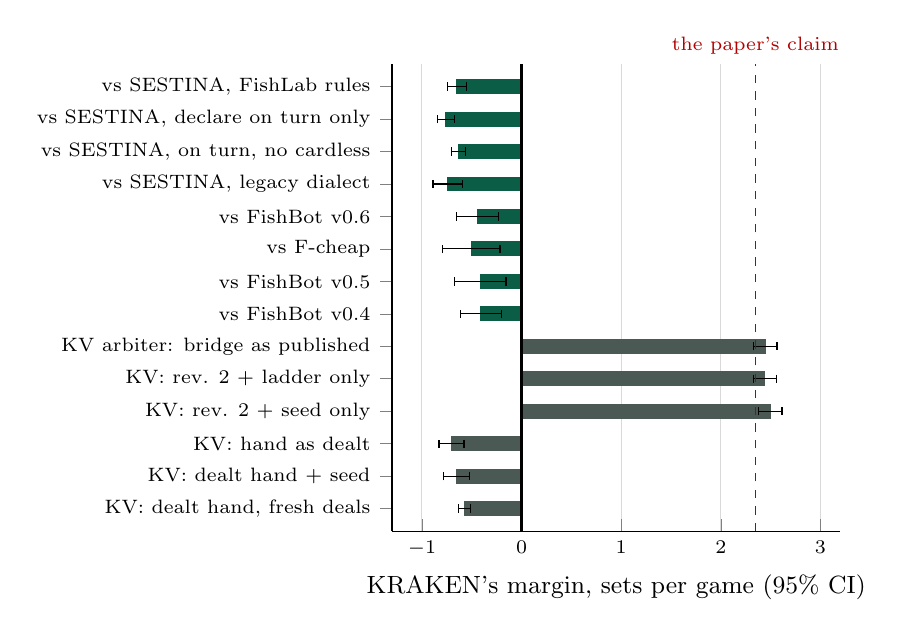
\begin{tikzpicture}
\begin{axis}[xbar, bar shift=0pt, width=0.6\linewidth, height=0.62\linewidth, xmin=-1.3, xmax=3.2,
  ymin=-0.7, ymax=13.7, ytick={0,1,2,3,4,5,6,7,8,9,10,11,12,13}, yticklabels={{KV: dealt hand, fresh deals}, {KV: dealt hand + seed}, {KV: hand as dealt}, {KV: rev. 2 + seed only}, {KV: rev. 2 + ladder only}, {KV arbiter: bridge as published}, {vs FishBot v0.4}, {vs FishBot v0.5}, {vs F-cheap}, {vs FishBot v0.6}, {vs SESTINA, legacy dialect}, {vs SESTINA, on turn, no cardless}, {vs SESTINA, declare on turn only}, {vs SESTINA, FishLab rules}},
  xlabel={KRAKEN's margin, sets per game (95\% CI)}, yticklabel style={font=\scriptsize}, xticklabel style={font=\scriptsize}, xlabel style={font=\small},
  bar width=5pt, axis lines*=left, xmajorgrids, grid style={gray!30}, clip=false,
  error bars/x dir=both, error bars/x explicit, error bars/error bar style={black}, error bars/error mark options={rotate=90, mark size=1.5pt}]
\addplot[fill=fishgreen, draw=fishgreen] coordinates {
  (-0.4067,6) +- (0.2060,0)
  (-0.4156,7) +- (0.2595,0)
  (-0.5056,8) +- (0.2895,0)
  (-0.4400,9) +- (0.2097,0)
  (-0.7393,10) +- (0.1492,0)
  (-0.6320,11) +- (0.0682,0)
  (-0.7587,12) +- (0.0829,0)
  (-0.6481,13) +- (0.0917,0)
};
\addplot[fill=fishgray, draw=fishgray] coordinates {
  (-0.5703,0) +- (0.0620,0)
  (-0.6530,1) +- (0.1262,0)
  (-0.7030,2) +- (0.1254,0)
  (2.4940,3) +- (0.1201,0)
  (2.4430,4) +- (0.1186,0)
  (2.4460,5) +- (0.1185,0)
};
\draw[thick] (axis cs:0,-0.7) -- (axis cs:0,13.7);
\draw[dashed, red!70!black] (axis cs:2.3466,-0.7) -- (axis cs:2.3466,13.7) node[above, font=\scriptsize, text=red!70!black] {the paper's claim};
\end{axis}
\end{tikzpicture}

\caption{KRAKEN's margin in every non-control cell of both arbiters, sets per game with 95\pct{}
intervals. Green: FishLab's arbiter. Grey: KV's arbiter, from the bridge as published (top three) to
the repaired bridge (bottom three). The dashed line is the paper's headline. The KV FishBot v0.6 cells
are in Table~\ref{tab:fishlab} only, since their bars would be that bot's margin, not KRAKEN's.}
\label{fig:margins}
\end{figure}

\subsection{KV's arbiter reproduces the paper}
\label{sec:kv}

With their engine, their rules and their bridge as published, on fresh deals, KRAKEN's margin is
$\kcVRevTwoMargin$~$[\kcVRevTwoLo, \kcVRevTwoHi]$ over \kcVRevTwoGames{} games, with
\kcVRevTwoSetShare\pct{} of sets and \kcVRevTwoWin\pct{} of games (first row of
Table~\ref{tab:kvarena}). The paper's journal gives $\kcMegaMargin$, \kcMegaSetShare\pct{} and
\kcMegaWin\pct{}. \sestina{} declares correctly \kcVRevTwoDeclS\pct{} of the time here against
\kcMegaDeclS\pct{} there, and hits \kcVRevTwoAskS\pct{} of its asks against \kcMegaAskS\pct{}. The
paper's measurement is therefore reproducible on its own apparatus, and the disagreement with
Section~\ref{sec:fishlab} is not noise on either side.

The instrumented rows say where the wrong declarations of \sestina{} come from. \sestina{} is forced to
declare \kcVRevTwoForcedPerGame{} times a game and gets \kcVRevTwoForcedS\pct{} of those right; its
\emph{voluntary} declarations, the ones its own gate chose to make, are right only
\kcVRevTwoVolS\pct{} of the time. Of its wrong declarations, \kcVRevTwoOwnErr{} per game are
ownership errors --- half-suits an opponent still held a card of --- against \kcVRevTwoAllocErr{}
allocation errors. Natively, the gate of \sestina{} essentially never declares a half-suit an opponent
holds a card of; something is wrong with what it is being told about the table.

\subsection{One line of the bridge}
\label{sec:variants}

\begin{table}[!ht]
\caption{Bridge variants inside KV's arbiter. All rows but the last are the same \kcVRevTwoGames{}
games (1,000 deals $\times$ 2 parities, same deal and agent seeds), so the paired column is a per-game
difference on identical deals. ``K'' is KRAKEN, ``S'' is \sestina{}.}
\label{tab:kvarena}
\small
\begin{tabularx}{\linewidth}{Q{1.6}N{0.75}N{1.25}N{0.8}N{0.75}N{0.7}N{0.85}N{1.3}}
\toprule
bridge & games & K margin & K wins & S decl.\ acc. & S ask hit & S own.\ err.\ per game & paired $\Delta$ vs rev.~2 \\
\midrule
as published (rev.~2) & \kcVRevTwoGames{} & \ci{$\kcVRevTwoMargin{}$}{\kcVRevTwoLo{},\,\kcVRevTwoHi{}} & \kcVRevTwoWin{}\% & \kcVRevTwoDeclS{}\% & \kcVRevTwoAskS{}\% & \kcVRevTwoOwnErr{} & --- \\
\textbf{hand as dealt} instead of current hand & \kcVDealtGames{} & \ci{$\kcVDealtMargin{}$}{\kcVDealtLo{},\,\kcVDealtHi{}} & \kcVDealtWin{}\% & \kcVDealtDeclS{}\% & \kcVDealtAskS{}\% & \kcVDealtOwnErr{} & \ci{$\kcVDealtPaired{}$}{\kcVDealtPairedLo{},\,\kcVDealtPairedHi{}} \\
rev.~2 + forced-endgame ladder only & \kcVLadderGames{} & \ci{$\kcVLadderMargin{}$}{\kcVLadderLo{},\,\kcVLadderHi{}} & \kcVLadderWin{}\% & \kcVLadderDeclS{}\% & \kcVLadderAskS{}\% & \kcVLadderOwnErr{} & \ci{$\kcVLadderPaired{}$}{\kcVLadderPairedLo{},\,\kcVLadderPairedHi{}} \\
rev.~2 + per-decision seed only & \kcVSeedGames{} & \ci{$\kcVSeedMargin{}$}{\kcVSeedLo{},\,\kcVSeedHi{}} & \kcVSeedWin{}\% & \kcVSeedDeclS{}\% & \kcVSeedAskS{}\% & \kcVSeedOwnErr{} & \ci{$\kcVSeedPaired{}$}{\kcVSeedPairedLo{},\,\kcVSeedPairedHi{}} \\
dealt hand and per-decision seed & \kcVDealtSeedGames{} & \ci{$\kcVDealtSeedMargin{}$}{\kcVDealtSeedLo{},\,\kcVDealtSeedHi{}} & \kcVDealtSeedWin{}\% & \kcVDealtSeedDeclS{}\% & \kcVDealtSeedAskS{}\% & \kcVDealtSeedOwnErr{} & \ci{$\kcVDealtSeedPaired{}$}{\kcVDealtSeedPairedLo{},\,\kcVDealtSeedPairedHi{}} \\
dealt hand, fresh deals (unpaired) & \kcVDealtBigGames{} & \ci{$\kcVDealtBigMargin{}$}{\kcVDealtBigLo{},\,\kcVDealtBigHi{}} & \kcVDealtBigWin{}\% & \kcVDealtBigDeclS{}\% & \kcVDealtBigAskS{}\% & \kcVDealtBigOwnErr{} & --- \\
\bottomrule
\end{tabularx}

\end{table}

Table~\ref{tab:kvarena} prices each hypothesis. The forced-endgame ladder --- the mechanism the
paper's own bridge repair addressed --- is worth $\kcVLadderPaired$~$[\kcVLadderPairedLo,
\kcVLadderPairedHi]$: nothing. A varying seed is worth $\kcVSeedPaired$~$[\kcVSeedPairedLo,
\kcVSeedPairedHi]$: nothing. Passing the hand as dealt is worth $\kcVDealtPaired$~$[\kcVDealtPairedLo, \kcVDealtPairedHi]$ sets per game, and it reverses the sign of the result:
KRAKEN's margin becomes $\kcVDealtMargin$~$[\kcVDealtLo, \kcVDealtHi]$, its share of games
\kcVDealtWin\pct{}. \sestina{}'s declaration accuracy rises from \kcVRevTwoDeclS\pct{} to
\kcVDealtDeclS\pct{} (voluntary \kcVDealtVolS\pct{}), its ownership errors fall from
\kcVRevTwoOwnErr{} to \kcVDealtOwnErr{} per game, and its ask hit rate rises from
\kcVRevTwoAskS\pct{} to \kcVDealtAskS\pct{} --- the same corruption was costing it asks as well as
declarations. Adding the varying seed on top changes little ($\kcVDealtSeedMargin$). On
\kcVDealtBigGames{} further fresh games the repaired bridge gives $\kcVDealtBigMargin$~$[\kcVDealtBigLo, \kcVDealtBigHi]$.

Two things follow. First, KV's arbiter and FishLab's now agree. Under the FishLab dialect closest to
KV's --- declaration on turn only, no cardless declaration --- FishLab gives $\kcENoootNcMargin$~$[\kcENoootNcMarginLo, \kcENoootNcMarginHi]$, against $\kcVDealtMargin$ and $\kcVDealtBigMargin$
from the repaired bridge in KV's arbiter; the remaining differences of hosting are discussed in
Section~\ref{sec:faithful}. Second, the
paper's mechanism story --- that \sestina{} finds cards at a comparable rate but does not know when a
half-suit is finished --- is describing a policy whose posterior had been corrupted before it was asked
anything. Its \kcMegaDeclS\pct{} is the bridge, not the engine.

\subsection{The same defect, decision by decision}
\label{sec:probe}

\begin{table}[!ht]
\caption{The decision probe: \kcPrGames{} games, \kcPrDecisions{} on-turn decisions of native
\sestina{} in FishLab's arbiter under KV's rules, each also answered by KV's shim from the current hand
and from the hand as dealt. Hypothetical declarations are scored against the true hands.}
\label{tab:probe}
\small
\begin{tabularx}{\linewidth}{Q{1.75}N{0.65}N{0.8}N{0.8}}
\toprule
 & native SESTINA & shim, current hand (rev.~2) & shim, hand as dealt \\
\midrule
declarations over these decisions & \kcPrNativeDecl{} & \kcPrCurDecl{} & \kcPrDealtDecl{} \\
of which wrong & \kcPrNativeWrong{} (\kcPrNativeWrongPct{}\%) & \kcPrCurWrong{} (\kcPrCurWrongPct{}\%) & \kcPrDealtWrong{} (\kcPrDealtWrongPct{}\%) \\
agrees with native on declare\,/\,not & --- & \kcPrCurAgree{} (\kcPrCurAgreePct{}\%) & \kcPrDealtAgree{} (\kcPrDealtAgreePct{}\%) \\
declares when native does not & --- & \kcPrCurOnly{} & \kcPrDealtOnly{} \\
\quad of which wrong & --- & \kcPrCurOnlyWrong{} & \kcPrDealtOnlyWrong{} \\
\quad naming a half-suit an opponent holds & --- & \kcPrCurOnlyOwn{} & \kcPrDealtOnlyOwn{} \\
declines when native declares & --- & \kcPrCurNativeOnly{} & \kcPrDealtNativeOnly{} \\
both declare, different allocation & --- & \kcPrCurBothDiff{} & \kcPrDealtBothDiff{} \\
same ask as native (of \kcPrAskCompared{}) & --- & \kcPrCurAsk{} (\kcPrCurAskPct{}\%) & \kcPrDealtAsk{} (\kcPrDealtAskPct{}\%) \\
first decision of a game identical, agents rebuilt per game (of \kcPrFreshFirst{}) & --- & \kcPrFreshFirstCur{} & \kcPrFreshFirstDealt{} \\
\quad agents reused across deals (of \kcPrFirst{}) & --- & \kcPrFirstCur{} & \kcPrFirstDealt{} \\
\bottomrule
\end{tabularx}

\end{table}

Table~\ref{tab:probe} removes the arbiter from the question altogether. Given the current hand, KV's
shim declares \kcPrCurDecl{} times where the native agent declares \kcPrNativeDecl{}; \kcPrCurWrongPct\pct{}
of the shim's declarations are wrong against \kcPrNativeWrongPct\pct{} of the native agent's, and of the
\kcPrCurOnly{} declarations the shim makes when the native agent does not, \kcPrCurOnlyWrong{} are
wrong and \kcPrCurOnlyOwn{} name a half-suit an opponent is holding. Given the hand as dealt, the shim
never declines a declaration the native agent makes and never allocates one differently; its
remaining excess declarations (\kcPrDealtOnly{}, \kcPrDealtOnlyWrong{} wrong) and the ask
disagreements are consistent with the restarted random stream, the one piece of state a fresh process
cannot reconstruct, and the seed schedule itself is priced at $\kcVSeedPaired$ in play. The
first-decision row is the check on everything else in their serialisation: with the native agents
rebuilt for every game, both versions of the shim answer what the native agent answers at all
\kcPrFreshFirst{} first decisions. With the agents reused across deals, \kcPrFirstDealt{} of
\kcPrFirst{} agree; the one exception is a first decision at which the reused native agent itself
differs from a freshly built one --- the cross-deal residual of \sestina{}'s report --- and at which
the shim matches the fresh agent, so it is a property of FishLab's harness, not of the bridge.

\section{The defect}
\label{sec:defect}

\subsection{What the bridge sends}

Their \code{Observation.from\_state} sets \code{hand = state.hands[player]}, the hand at this moment,
and \code{DylanV07.\_feed} writes it to the \code{HAND} line. Their shim then boots the agent with
\code{agent->reset(seat, hand, rules, seed)} and replays the history. In FishLab, \code{reset} is
called once, by \code{Game::setup}, with the hand as dealt, and the agent thereafter learns every
movement from the events it observes. The two conventions coincide only until the seat's first
transfer.

\subsection{What the engine does with it}

\code{Knowledge::init} (\code{engine/src/belief.hpp}) marks every card in the reset hand as owned by
this seat and every other card as unknown with a candidate set that excludes this seat. Under the
bridge's convention a card this seat has since taken from an opponent is therefore ``mine since the
deal'', and a card it was dealt and has since lost is ``never mine''.

The damage is done when the history is replayed. \code{Knowledge::onEvent}
(\code{belief.hpp:\kcBeliefCertLines}) turns every ask by a seat $p$ in half-suit $S$ into a legality
certificate --- $p$ held some other card of $S$ at that moment --- built over the cards of $S$ whose
owner is still unknown and whose candidate set includes $p$ (lines \kcBeliefCertLines{}, verbatim):
\begin{lstlisting}
  // (C5): the asker held another card of S.  Vacuous if we already know one.
  bool vacuous = false;
  uint64_t D = 0;
  for (int i = 0; i < SETSZ; i++) {
    int d = cardOf(S, i);
    if (d == e.card) continue;
    if (owner[d] == e.actor) { vacuous = true; break; }
    if (owner[d] == UNKNOWN && (mask[d] & (1u << e.actor))) D |= bit(d);
  }
  exclude(e.card, e.actor);                          // (C3) asker lacks the card
  if (!vacuous && D) {
    if (__builtin_popcountll(D) == 1) setOwner(__builtin_ctzll(D), e.actor);
    else if (!dedupDisj) disj.push_back(Disjunction{uint8_t(e.actor), D});
\end{lstlisting}

Suppose KRAKEN's seat $p$ asks for a card of $S$ at ply 10, holding only the 3 of that suit, and at ply
40 \sestina{}'s seat takes that 3 from $p$. At the reconstruction for any decision after ply 40 the 3
is already \code{owner == me}, so when ply 10 is replayed it is excluded from $D$. The certificate is
now a statement about the wrong cards; if only one card of $S$ remains unknown with $p$ in its
candidate set, line~\kcBeliefPinLine{} pins that card to $p$ as a deduction --- a card $p$ never
held. The exact counting and the Sinkhorn fit that \sestina{}'s declaration gate reads then reconcile a
constraint set no deal satisfies, and the reconciliation shows up as ownership errors: half-suits
declared as wholly held while an opponent still holds a card of them.

\subsection{Why every check passed}

The paper's checks could not see this, for three reasons. \emph{Legality}: every move the shim
returns is legality-checked and zero fallbacks are reported, but a policy with a corrupted belief
still makes legal moves. \emph{Decision-level verification was done for the other bridge}: the
fresh-agent comparison of the paper's Appendix~C (\kcPaperShimDecisions{} decisions, no mismatches)
verifies KRAKEN's own transport, \code{fish4/decide.py}, against a fresh KRAKEN agent; for the v0.7
shim the paper and its bridge README report legality checks, the fallback counter, twenty mixed games
with zero fallbacks, and a unit test of the forced-half-suit rule (\code{tests4/test\_dylan\_bridge.py},
fetched upstream), none of which compares a decision with what the native agent would have done. A
test in the shape of Appendix~C would not have caught it either unless the fresh agent were the
\emph{native} one: a fresh agent booted from the same current hand reproduces the defect and compares
it with itself. \emph{Forensics}: the paper examined \sestina{}'s errors closely (\S11.9) and found
that every one of the \kcPaperNeverMoved{} cards inside its ownership errors had never publicly moved;
that ownership errors were \kcPaperRateRatio{} times as frequent, per ply of exposure, in half-suits
KRAKEN had asked in as in half-suits it had not; and that of the declarations which followed both an
ask by KRAKEN and a later capture of a card of that half-suit by \sestina{},
\kcPaperFollowedBothPct\pct{} were ownership-wrong, against \kcPaperFollowedTakingPct\pct{} for a
capture alone. That is exactly the population this defect produces: KRAKEN's ask creates the
certificate, \sestina{}'s later capture in that half-suit is what the current-hand reset mis-files, and
the phantom deduction lands on a card that never moved. The paper read the signature as a flaw in
\sestina{}'s inference (``as though `at least one' had been `exactly one'\,''); it is not what the code
does.

\subsection{What inherits it}

Every cross-engine figure in the paper was taken through this bridge: the head-to-head, the
declaration decomposition (\kcPaperDeclShare\pct{} of the margin as ``declaration accounting''), the
acquisition and turn-count tables, the README's dialect gaps, the pre-registered foreign-opponent
checks R2 and R6, and the contestation-term port of Table~18, which measured a FishLab coordinate
against a corrupted FishLab. Their website's exhibition reconstructs every session from the public log
through the same \code{\_feed}. The paper's bridge ledger defends the paired contrasts among these
--- the dialect gaps, R2, R6 --- as bridge-independent because every arm shared the bridge. That holds
only when the bridge's effect is additive, and a corruption of the opponent's posterior worth three
sets a game is not: the README's own table has off-turn declaration costing KRAKEN $\kcReadmeOffturnGap$
sets against the corrupted \sestina{}, while against the native one in FishLab it is worth
$\kcEOffturnGap$ to KRAKEN (Table~\ref{tab:fishlab}). A gap measured against a corrupted opponent is
not the gap against the real one. The bridge-revision-2 repair the paper describes is real but
immaterial by comparison: it addressed which half-suit a forced best guess names, worth
$\kcPaperBridgeBugPrice$ by the paper's own pairing and $\kcVLadderPaired$ for the whole ladder here.

\section{Discussion}
\label{sec:discussion}

\subsection{What is refuted, what stands, what was not tested}

Refuted: that KRAKEN beats \sestina{} by about $\kcMegaMargin$ sets per game, takes \kcMegaSetShare\pct{}
of sets, wins \kcMegaWin\pct{} of games, or has an eighteen-point declaration-accuracy edge over it.
In both arbiters, once the bridge passes \sestina{} the hand it was dealt, KRAKEN loses by roughly
$\kcVDealtBigMargin$ to $\kcENoootMargin$ sets per game under each of the dialects tested (four in
FishLab, KV's baseline in KV's arbiter) and wins about two games in five. The
mechanism story built on the \kcMegaDeclS\pct{} row is refuted with it.

Standing: everything in the paper that does not pass through the bridge. Its internal lineage result
($\kcPaperVthreeMargin$ sets per pair against its own v0.3 champion), its exact counting and
sampling, its posterior-quality measurements, its endgame solver and its pre-registration discipline
are untouched by anything here, and this report makes no claim about them.

Not claimed: a global ranking. One foreign opponent is one opponent, and \sestina{}'s own report
declines the same claim for the same reason. KRAKEN's placement below FishBot v0.4 through v0.6 on
FishLab's ladder is context, not a leaderboard.

\subsection{Which arbiter is faithful}
\label{sec:faithful}

Neither arbiter is the game; each hosts one bot natively and the other through a bridge, and the
question is what each bridge costs. KRAKEN is stateless by design --- its guide says a host may send
one line and close the pipe --- so a bridge costs it nothing, and in FishLab it is additionally handed
the true holders on a wrong declaration and declares more accurately than in its own arbiter.
\sestina{} is stateful and searches; a fresh process per decision restarts its random stream, their
forced endgame lets only the mover declare and from a best guess, and it is never polled off-turn.
Even with the dealt hand, the probe shows the shim still declaring wrongly \kcPrDealtWrongPct\pct{} of
the time against \kcPrNativeWrongPct\pct{} natively. \sestina{}'s ask hit rate in the repaired KV
arbiter (\kcVDealtAskS\pct{}) is not below FishLab's under the matched dialect
(\kcENoootNcAskB\pct{}), so no residual shows there. Of the hosting differences, the two that could be
varied one at a time are priced in Table~\ref{tab:kvarena} and are small; the rest are bounded only by
the end-to-end comparison of matched-dialect cells in Section~\ref{sec:variants}. The honest summary is
that the corrected KV arbiter and FishLab give the same sign and nearly the same size, and that what
little residual there is runs against \sestina{} rather than for it.

\subsection{Fairness to KRAKEN in FishLab}

The symmetric question is whether \code{kv6.hpp} does to KRAKEN what \code{dylan\_v07.py} did to
\sestina{}. The evidence that it does not: KRAKEN's three stated requirements are met;
its own event-stream checker never rejected a position; the transcript of a full deal is well-formed;
it is handed information FishLab's own agents do not get; it has no clock; the harness is symmetric;
and its declaration accuracy is higher here than at home. Two things are not evidence and are not
claimed as such: the mirror cell cannot see a defect that hits both copies equally, and no
decision-level probe of KRAKEN's hosting was built. Two asymmetries remain. A cardless KRAKEN seat is
not asked to declare on its own turn, because KRAKEN's on-turn loop does not implement cardless
declaration, though it is still polled off-turn; the \flag{no-cardless-declare} cell removes that
rule for both sides at once and moves the result by $\kcECardlessShift$ in KRAKEN's favour on
different deals, within the battery's unpaired resolution. And in
FishLab's forced endgame, when KRAKEN's own decision names a different half-suit from the one the
ladder's last rung demands, the engine's default all-to-one-seat guess is applied in KRAKEN's name and
counted; that counter is not printed by the match driver, so it is bounded here instead: KRAKEN makes
\kcENoootForcedPerGame{} forced declarations a game under its own dialect at \kcENoootForcedAcc\pct{}
accuracy (\kcEDefaultForcedPerGame{} at \kcEDefaultForcedAcc\pct{} under FishLab's), so even if every
wrong one were such a substitution the effect is at most \kcENoootFallbackBound{} sets per game
(\kcEDefaultFallbackBound{} under FishLab's rules), which does not reach the result. If KV's project
finds a defect in \code{kv6.hpp} the way this report found one in theirs, the paired instrument to
price it is the same one used here.

\subsection{What a cross-engine measurement should require of its bridge}

The general lesson is the one the paper itself states and then did not apply: a number measured
through a bridge is a claim about the bridge. Four checks would have caught this defect, and any of
them is cheap.
\begin{enumerate}
\item \textbf{Reconstruct against the native agent, not against a copy of the reconstruction.} At
      the first decision of a game, a fresh agent and the live agent have identical state; they must
      answer identically, and the comparison must be made on positions from real games, after
      transfers have happened.
\item \textbf{Round-trip every reconstructed input.} A hand handed to \code{reset} must, replayed
      forward through the history, reproduce the hand the arbiter holds. This is one line and fails
      loudly.
\item \textbf{Host in both directions and require agreement.} Two independently written engines
      that disagree by three sets a game on the same pairing are reporting a bridge defect, not a
      dialect.
\item \textbf{Account for errors by class.} A foreign bot that suddenly declares half-suits its
      opponents hold is not exhibiting a subtle inference weakness; it is being lied to. Ownership
      versus allocation errors, and forced versus voluntary declarations, separate the two in one
      table.
\end{enumerate}
Legality checks and fallback counters, the checks the paper relied on, are necessary and not
sufficient: a scrambled belief plays legal moves.

\section{Conclusion}

KRAKEN v1.1's cross-engine headline is an artifact of its bridge into \sestina{}, which reset the
opponent with the hand it held rather than the hand it was dealt and thereby corrupted every
certificate the opponent's belief is built from. The paper's number reproduces on its own apparatus;
correcting one line and replaying the same deals moves it by $\kcVDealtPaired$ sets per game and
reverses its sign; FishLab's arbiter, with KRAKEN hosted exactly as its guide demands, gives the same
answer independently; and the defect is visible decision by decision. Under each of the dialects tested,
\sestina{} beats KRAKEN by roughly two thirds of a set per game and wins about three games in five, and KRAKEN sits below every FishBot release since v0.4. A patch for their bridge
accompanies this report.

\appendix

\section{Reproduction and artifacts}

FishLab is at \url{https://github.com/dylann4500/fishbot}; this report was produced at commit
\code{f9b4743} with the uncommitted additions in the working tree at the time, none of which touch the
measured engine core. KV's repository is at
\url{https://github.com/kv1514/fish-researchp12}
(branch \code{claude/fishnbot-work-access-g7ciey}, head \code{\kcUpstreamHead}). All artifacts, drivers and this document's number generator are under
\code{research/kraken-check/}:
\begin{description}
\item[\code{e1\_results.jsonl}] one row per FishLab block, with the exact command line;
      \code{run\_e1.py} regenerates it.
\item[\code{e2\_*.jsonl}] one row per game in KV's arbiter, per bridge variant, with per-side ask,
      declaration, forced-declaration and error-class counts; \code{kvarena/run\_e2.py} and
      \code{kvarena/e2\_variants.py} regenerate them after \code{stage\_kvarena.sh} has copied KV's
      package into a work directory and compiled their shim (and the ladder-capable
      \code{shim\_decide2.cpp}) against \code{engine/src}.
\item[\code{e5\_probe.json}, \code{agree\_probe.cpp}] the decision probe.
\item[\code{e4\_upstream\_777001.json}] upstream KRAKEN v1.1 on the vendored block's seed.
\item[\code{bridge\_kraken.jsonl}] a full request--reply transcript of \code{kv6.hpp} for one deal.
\item[\code{upstream/}] the paper's headline result and 10,000-game journal, the bridge ledger, and
      the bridge file the patch applies to.
\item[\code{dylan\_v07\_dealt\_hand.patch}] the repair (bridge revision~3).
\item[\code{analyse.py}, \code{make\_numbers.py}, \code{make\_report.py}] the aggregation, the
      macros and tables of this document, and the Markdown report \code{docs/KRAKEN-CLAIM-CHECK.md}.
\end{description}
The commands, from the repository root:
\begin{lstlisting}
python3 research/kraken-check/run_e1.py 9   # argument = threads (no effect on results)
sh research/kraken-check/stage_kvarena.sh && cd engine/external/kvarena-work
PY=../kv-venv/bin/python
OUT=../../../research/kraken-check
E2_VARIANT=rev2      $PY run_e2.py 1000 6 910000 $OUT/e2_rev2.jsonl
E2_VARIANT=dealthand $PY run_e2.py 1000 6 910000 $OUT/e2_dealthand.jsonl
for v in ladder seedvary dealtseed; do
  E2_VARIANT=$v $PY run_e2.py 1000 6 910000 $OUT/e2_$v.jsonl; done
E2_VARIANT=dealthand $PY run_e2.py 4000 10 920000 $OUT/e2_dealthand_big.jsonl
sh $OUT/run_probe.sh                        # the decision probe (e5)
cd ../../..
python3 research/kraken-check/analyse.py
python3 research/kraken-check/make_numbers.py
\end{lstlisting}

\section{The repair}

The whole of the patch to \code{fish4/dylan\_v07.py} is the following method and its use in
\code{\_feed} in place of \code{obs.hand}:
\begin{lstlisting}
@staticmethod
def _dealt_hand(obs):
    me, hand = obs.player, obs.hand
    for ev in reversed(obs.history):
        if isinstance(ev, AskEvent) and ev.success:
            if ev.asker == me:      hand &= ~(1 << ev.card)
            elif ev.target == me:   hand |=  (1 << ev.card)
        elif isinstance(ev, ClaimEvent):
            base = ev.half_suit * CARDS_PER_HALF_SUIT
            for i, holder in enumerate(ev.revealed):
                if holder == me:    hand |=  (1 << (base + i))
    return hand
\end{lstlisting}
KV's own \code{Observation} class already provides exactly this walk as \code{initial\_hand()}, used by
their information-leakage test, so the repair is also the one-token change \code{obs.hand} to
\code{obs.initial\_hand()} in \code{\_feed}; the patch spells the walk out so that it does not depend
on that helper. It uses only public events and the seat's own hand, so it is available to any host; a host whose
engine does not reveal holders on a failed declaration can substitute the declared holders for a
successful one and the seat's own knowledge of which of its cards were retired for a failed one.

\begin{thebibliography}{9}
\bibitem{kraken} Kausthubh Veldanda. \emph{Exact Inference Is Not Enough: Opponent Models and Endgames
in Six-Player Literature}. KRAKEN v1.1, 30 August 2026. \code{paper/kraken.pdf} in the repository\\
\url{https://github.com/kv1514/fish-researchp12}.
\bibitem{sestina} Dylan Nguyen. \emph{SESTINA v1.0: Exact Inference, Robust Evaluation, and
Adversarial Testing in Six-Player Canadian Fish}. FishLab technical report, 31 August 2026.
\code{output/pdf/sestina\_v10.pdf} in the repository\\
\url{https://github.com/dylann4500/fishbot}.
\end{thebibliography}

\end{document}
